\documentclass[letterpaper, 12pt]{math}

\usepackage{amsmath}
\usepackage{amssymb}
\usepackage{tikz}

\title{Sets}
\author{Alvin Lin}
\date{Discrete Math for Computing: January 2017 - May 2017}

\begin{document}

\maketitle

\section*{Sets}
\textbf{Sets} are fundamental discrete structures. A set is an unordered
collection of objects called \textbf{elements} of the set. A set is said
to contain its elements. We write \( a \in A \) if \( a \) is an element of the
set \( A \). We write \( a \notin A \) if \( a \) is not an element of the set
\( a \). Sets are usually given in uppercase letters while elements are
generally given in lowercase letters. \par
There are several ways to describe sets:
\begin{enumerate}
  \item Roster method
  \item Set builder notation
  \item Venn diagrams
\end{enumerate}

\subsection*{Roster Notation}
The set of all vowels is:
\[ V = \bigg\{a,e,i,o,u\bigg\} \]
The set of all odd positive integers less than 12 is:
\[ O = \bigg\{1,3,5,7,9,11\bigg\} \]
Other examples:
\[ U = \bigg\{dog,cat,fish\bigg\} \]
\[ dog \in U \]
\[ chicken \notin U \]

\subsection*{Set Builder Notation}
\[ O = \bigg\{x|x\ is\ an\ odd\ positive\ integer\ less\ than\ 100\bigg\} \]
\begin{align*}
  [a,b] &= \bigg\{x|a \leq x \leq b \bigg\} \\
  (a,b] &= \bigg\{x|a < x \leq b \bigg\} \\
  [a,b) &= \bigg\{x|a \leq x < b \bigg\} \\
  (a,b) &= \bigg\{x|a < x < b \bigg\}
\end{align*}

\subsection*{Set Equality}
Two sets are equal if and only iff they contain the same elements. Thus \( A \)
and \( B \) are equal if:
\[ \forall{x}(x \in A \leftrightarrow x \in B) \]
We write \( A = B \) when sets are equal.
\[ \bigg\{1,2,3\bigg\} = \bigg\{3,1,2\bigg\} \]
\[ \bigg\{1,2,3\bigg\} \neq \bigg\{1,2,4\bigg\} \]

\subsection*{Venn Diagrams}
Venn Diagrams are useful for showing relations between sets. The universal
set \( U \) contains all elements. The set \( V \) contains the set of all
vowels.
\begin{center}
  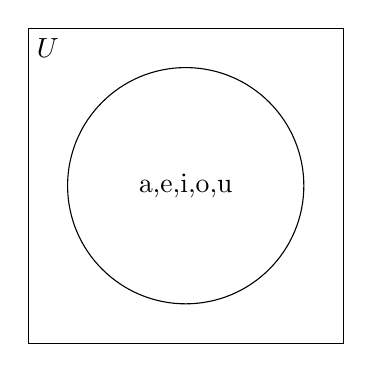
\begin{tikzpicture}
    \draw (0,0) -- (4,0) -- (4,4) -- (0,4) -- (0,0);
    \draw (2,2) circle (1.5cm);
    \node at (2,2) {a,e,i,o,u};
    \node at (0.25,3.75) {\( U \)};
  \end{tikzpicture}
\end{center}

\subsection*{Subsets}
The set \( A \) is a subset of the set \( B \) if and only if every element of
\( A \) is also in \( B \), notated as \( A \subseteq B \)
\[ \forall{x}(x \in A \to x \in B) \]
\[ \bigg\{1,2,3\bigg\} \subseteq \bigg\{1,2,3,4\bigg\} \]
\[ \bigg\{1,2,4\bigg\} \subseteq \bigg\{1,2,5\bigg\} \]

\subsection*{The Empty Set}
The empty set \( \emptyset \) is the set consisting of no elements (null set).
\par
\textbf{Theorem:} If \( S \) is a set, then \( \emptyset \subseteq S \) and
\( S \subseteq S \).

\begin{center}
  If you have any questions, comments, or concerns, please contact me at
  alvin@omgimanerd.tech
\end{center}

\end{document}
